\chapter{Introducción}
\label{chap:intro}

\drop{A}{ctualmente} existen numerosos avances en lo que a las <<nuevas tecnologías>> se refiere y cada vez tenemos más dispositivos con los que comunicarnos y estar en contacto con amigos, familiares o conocidos en todo momento. Estas nuevas formas de comunicación están presentes en todos los ámbitos y han modificado la forma de relacionarse. Uno de los ámbitos en los que ha sucedido esto es el educativo. Por ejemplo, antes se recurría al reparto de una circular para anunciar ciertos eventos a los alumnos para que se la entregaran a los padres o tutores o escribir una nota en la agenda del alumno para que la entregase firmada al día siguiente si no había hecho los deberes asignados o había ocurrido algún percance. Posteriormente, se podría usar el correo electrónico para comunicarse directamente con los padres, asegurándose de la correcta recepción del comunicado, aunque pudiera ocurrir que éstos no lo revisaran en tiempo y forma.

Existen multitud de aplicaciones <<generalistas>> de mensajería instantánea que se describirán con detalle a lo largo de este trabajo. La comunidad autónoma de Castilla-La Mancha posee la plataforma educativa llamada <<Papás 2.0>> (Figura \ref{fig:papas20}), que se encuentra más enfocada al sector educativo. Se trata de una plataforma educativa perteneciente a la Consejería de Educación, Cultura y Deportes de la \acf{JCCM} que facilita la gestión administrativa y establece una vía de comunicación entre los centros educativos y las familias, ofreciendo información relevante a los padres \cite{JCCM2017}. Además, permite llevar un seguimiento sobre las tareas, trabajos, controles, exámenes, faltas de asistencia y fechas de entrega \cite{JCCM2010}.

\begin{figure}[!h]
	\begin{center}
		
\includegraphics[width=0.4\textwidth]{/logo_papas_20}
		\caption{Logo de Papás 2.0}
		\label{fig:papas20}
	\end{center}
\end{figure}

\newpage

Papás 2.0 ofrece una serie de características que pueden resultar de gran valor para los padres, siendo éstas las más destacadas:

\begin{itemize}
	\item Visualizar los profesores que dan clase a los hijos con sus datos y posibilidad de escribir un mensaje directamente a cualquiera de ellos.
	\item Consultar las citas concertadas con los profesores, junto con la fecha, hora y motivo de la visita.
	\item Consultar el horario escolar.
	\item Consultar las faltas de asistencia, con la posibilidad de ser notificado vía SMS o correo electrónico. Del mismo modo, se podrá registrar una notificación cuando se sepa que el hijo va a faltar a ciertas horas.
	\item Consultar trabajos y tareas de cada hijo, así como ver las fechas de los exámenes y sus notas del curso y su trayectoria escolar.
	\item Envío y recepción de mensajes mediante grupos, pudiendo adjuntar archivos de tamaño no superior a 1 \acf{MB} y con un máximo de 3 \acs{MB} en total.
\end{itemize}

A pesar de que esta aplicación es de gran utilidad por las funcionalidades y facilidades que ofrece tanto a padres como a personal docente, se trata de una plataforma más cercana al correo electrónico que a una aplicación de mensajería instantánea, donde las personas sí que se comunican en tiempo real. En este último caso es donde toman especial relevancia los \textit{smartphones}, que se suelen llevar consigo y desde los que se puede acceder a casi cualquier servicio por estar permanentemente conectados a Internet. Por tanto, normalmente no se espera a tener un ordenador cerca para comunicarse con otras personas, sino que se hace uso directamente del teléfono móvil y de sus aplicaciones. Teniendo esto en cuenta, los profesores podrían comunicarse en tiempo real con los padres y éstos pueden aportar algún tipo de \textit{feedback} en un corto periodo de tiempo.

Aunque existen diversas soluciones para la comunicación entre los padres y el centro en el que se encuentren sus hijos y aportan numerosos beneficios a la comunidad educativa, muchas veces se pueden producir malentendidos cuando se hace uso de la mensajería instantánea, entre otros problemas produciéndose, además, situaciones poco deseables entre todos los miembros. Esto se debe a que se crean grupos de chat en los que el centro tiene poco o nada que ver, no se encuentran convenientemente controlados y, con el tiempo, puede ocurrir que la finalidad original se acabe desvirtuando.

\newpage

Un ejemplo de esa desvirtuación es este caso, donde un grupo de madres se negaba a llevar a sus hijos al colegio debido a que a la clase de éstos acudía un niño que sufría síndrome de Asperger. Sucedió en Buenos Aires, Argentina, y pronto se dio a conocer en Internet.
En las capturas de la conversación (Figura \ref{fig:whatasper}) se puede ver cómo las madres se alegran de que este chico fuera cambiado de clase. <<Una buenísima noticia>>, según indicaba una de las integrantes \cite{Vanguardia2017}.

\begin{figure}[!h]
	\begin{center}
		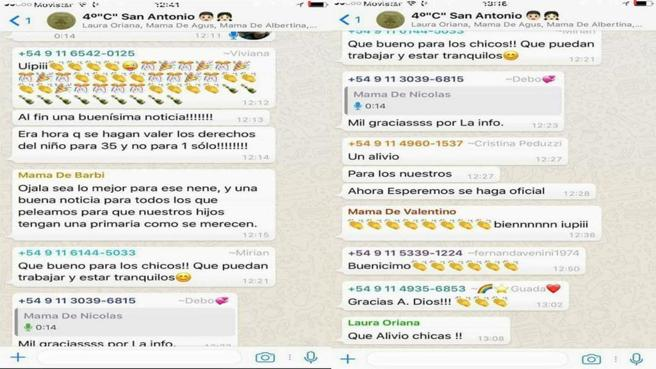
\includegraphics[width=0.8\textwidth]{/whatsapp_asperger}
		\caption{Captura conversación madres}
		\label{fig:whatasper}
	\end{center}
\end{figure}

Más allá de los problemas que puedan surgir entre los padres, los grupos pueden llegar incluso a dañar a los propios hijos. Esto puede suceder puesto que hay padres que comparten el trabajo realizado en casa para que otros niños o padres puedan beneficiarse de ello. Esta práctica puede repercutir en un mal aprendizaje del niño y, por tanto, en una disminución de su rendimiento escolar. Incluso pueden llegar a compartir fotos de los regalos colocados debajo del árbol en la época navideña \cite{Alias2017}. Por todo esto se debe establecer de manera firme y consensuada la figura del administrador del grupo, que será quien se encargue del cumplimiento y gestión de las normas para que la relación y saber estar de los padres no se quede sólo en el trato presencial sino que se extrapole a las nuevas soluciones digitales.

Un último caso es el de una madre que mandó una carta a una redactora. Sucedió en Argentina y en ella explica cómo, a raíz de abandonar el grupo de madres, éstas la tratan de una manera diferente debido a que en dicho grupo se hablaba demasiado, llegando a ser <<insoportables>>, decía la madre. Lo que pensaba se confirmó al necesitar a una madre para que recogiera a su hija, asegurando que le devolvería el favor la próxima vez. Esta madre leyó e ignoró el mensaje y, posteriormente, alegó que no se había dado cuenta \cite{Consuelo2017}.

\newpage

Las bondades de la mensajería instantánea son muy amplias y bien conocidas aunque, como en todo, se debe tener mesura en su uso y cierto control, sobre todo si se trata de temas más sensibles como la educación o los hijos. Por eso, en este trabajo fin de grado se plantea el desarrollo de una aplicación enfocada a este sector que evite, en la medida de lo posible, problemas como los descritos anteriormente.

%TODO: Explicar cada capítulo
\section{Estructura de la memoria}
A continuación se detalla la estructura de este trabajo fin de grado, que se encuentra dividido en varios capítulos:

\begin{definitionlist}	
	\item[Capítulo \ref{chap:intro}: \nameref{chap:intro}]
	
	\item[Capítulo \ref{chap:objetivos}: \nameref{chap:objetivos}]
	Finalidad y justificación (con todo detalle) del presente documento.
	
	\item[Capítulo \ref{chap:antecedentes}: \nameref{chap:antecedentes}]
	
	\item[Capítulo \ref{chap:metodologia}: \nameref{chap:metodologia}]
	
	\item[Capítulo \ref{chap:resultados}: \nameref{chap:resultados}]
\end{definitionlist}

% Local Variables:
%  coding: utf-8
%  mode: latex
%  mode: flyspell
%  ispell-local-dictionary: "castellano8"
% End: